\documentclass[12pt]{article}
\usepackage{lingmacros}
\usepackage{tree-dvips}
\usepackage{graphicx}

\begin{document}
\begin{center}
\section*{Introduction to Machine Learning}
\subsubsection*{Section 1}
\end{center}
\section*{Linear Algebra}
\subsection*{1.a}
$\Rightarrow$ 
symmetric matrix A is PSD such that ${v^tAv}$ $=$ ${(v^tu) diag (\lambda)(u^tv)}$  = \\
${\sum_{i}\lambda_i(Vu^t)^2\geq0}$ where $\lambda$ is the Eigenvalue of $A$. \\and matrix A can be decomposed as: \[A = 
 QDQ^t = Q*diag(\lambda_1,\lambda_2\ldots\lambda_n)*Q^t =\]  \[Q*diag(\sqrt{\lambda_1},\sqrt{\lambda_2}\ldots\sqrt{\lambda_n})*diag(\sqrt{\lambda_1},\sqrt{\lambda_2}\ldots\sqrt{\lambda_n})*Q^t= XX^t\]
\\\\
$\Leftarrow$ A can be written as $v^tXX^tv$ we get: \[ v^tAv=v^tXX^tv=(X^tv)^t(X^tv)=\parallel X^t_v \parallel \geq 0\]
\subsection*{1.b}
for a given PSD matrix A and $\mathbf \alpha\in{R}$    \\
(*) $v^t(\alpha A)\geq 0$ $\Rightarrow$ $v^t(u A)\geq 0$ when $u , A \geq 0$
\\then for  PSD matrix's A,B  when $A,B \geq 0$ , $A+B \geq 0$\\
now let's apply (*) on (A+B) we will get (**)
\[v^t(A+B)v=v^tAv+v^tBv \geq 0\]
then from both (*) and (**) immediately get $\alpha A+\beta B\geq 0$
\\
 the set of all n × n PSD matrices over ${R}$ is not a vector space over $R$ because its not apply the closures to multiplication in scalar property , for $\lambda < 0$ and 
 \[ A\geq 0 \rightarrow  \lambda A < 0 \rightarrow \lambda A \notin \lbrace PSD \rbrace \]
 
\section*{Calculus and Probability}
\subsection*{1.a}
for $x_1,x_2\ldots x_n$  i.i.d $U([0, 1])$ continuous random variables, lets write the  \\Order Statistics such as  $\overline{x_1} ,\overline{x_2}\ldots \overline{x_n}$ when $\forall$ i , $\overline{x_i} \leq \overline{x_{i+1}}$
first lets find the CDP of $Y=MAX\lbrace x_1,x_2\ldots x_n \rbrace=\overline{x_n}$ :\\
\[F_y(x)=F_{ \overline{x_n}}=\Pr(\overline{x_n}\leq k)=\Pr(\overline{x_1}\leq k,\overline{x_2}\leq k\ldots\overline{x_n}\leq k)\] because they i.i.d 
\[\Pr(\overline{x_1}\leq k)\Pr(\overline{x_2}\leq k)\ldots\Pr(\overline{x_n}\leq k)=[\Pr(\overline{x_i}\leq k)]^n=[F_x(k)]^n\]
\[(*)  F(x_i) = \left\{ \begin{array}{rcl}
{0} & \mbox{for}
& x<0 \\ x/1 & \mbox{for} & x\in\lbrace0,1\rbrace \\
1 & \mbox{for} & x>1
\end{array}\right.
f(x) = \left\{ \begin{array}{rcl}
{1} & \mbox{for}
& x\in\lbrace0,1\rbrace\\ 0 & \mbox{for} & x\notin\lbrace0,1\rbrace 
\end{array}\right.\] we get:
\[f_y(k)=f_{\overline{x_n}}(k)=\frac{d}{dk}(F_{\overline{x_n}}(k))^n=n(F(k))^{n-1}f(k)\] now lets set values in (*) and get :\\
\[f_y(k)=nk^{n-1}f(k)=nk^{n-1}f(k)=nk^{n-1}I_{(1,0)}\sim Beta(n,1)\]  therefore : 
\[ \lim(E[y])_{ n\to \inf}= \lim(\frac{n}{n+1})_{ n\to \infty}\longrightarrow 1\]
\\
 and : \[ (var[y])_{ n\to \inf}= \lim(\frac{n}{(n+1)^2(n+2)})_{ n\to \inf}\rightarrow 0 \]
\begin{center}
\includegraphics[scale=0.4]{beta.png} 
\end{center}
\subsection*{2}
\[E[|x-\alpha |] =  \int^{+\infty}_{-\infty} |x-\alpha |f(x) \, dx =  \int^{\alpha}_{-\infty} |x-\alpha |f(x) \, dx  + \int^{+\infty}_{\alpha} |x-\alpha |f(x) \, dx \] when $\alpha \in argmin$ :\\  \[\underbrace{(\alpha -x)f(x)|}_{\to 0}+ \int^{\alpha}_{-\infty} f(x) \, dx + \underbrace{(x-\alpha)f(x)|}_{\to 0}- \int^{+\infty}_{\alpha} f(x) \, dx\] \\
\[\displaystyle{\Rightarrow  \int^{\alpha}_{-\infty} f(x) \, dx =\int^{+\infty}_{\alpha} f(x) \, dx} \Rightarrow \Pr(x\leq \alpha)=\Pr(x\geq \alpha)\Leftrightarrow \] .\\\[ \ { \Pr(x\leq \alpha)=1/2}\]
\section*{Optimal Classifiers and Decision Rules}
\subsection*{1.a}
Let X and Y be random variables where Y can take values in $Y = \lbrace1, \dots, L\rbrace$, and Let $\ell$
be the 0-1 loss function defined in class , hence:   
\[E[\triangle(y,f(x))]= \sum_{k=1}^{L}Pr(X=\hat{x},Y=k)\triangle(k,f(x))  \] 
using bayes :
\[ \sum_{k=1}^{L}\Pr(X=\hat{x})\Pr(Y=k|X=\hat{x})\triangle(k,f(k))=\Pr(X=\hat{x})\sum_{k=1}^{L}\Pr(y=k|X=\hat{x})\triangle(k,f(k))\]
\[L(h)=Arg\min_{f:X\to Y}\lbrace\Pr(x=\hat{x})\sum_{y\neq k,y\in \lbrace1\ldots L\rbrace}\Pr(y=k|X=\hat{x})\rbrace=f(\hat{x})=h(x)=k
\]
\[\Rightarrow
h(\hat{x})=Arg\max\lbrace\Pr (x=\hat{x})(1-\Pr(y=k|X=\hat{x})\rbrace : h(\hat{x})=k
\]
\[ h(\hat{x})=Arg\max_{y\in Y} \Pr(y=i|x=\hat{x})
\]
\section*{Optimal Classifiers and Decision Rules}
\subsection*{1.b}
To find decision rule for:
\[ \Pr [y = 1 | X] > \Pr [y = 0 | X]\]
lets apply bayes  rule on 
both sides.
we get:
\[ \frac{f_{X|Y =1} (x) Pr [Y = y]
fX (X)}{f_x} > \frac{f_{X|Y =0} (x) Pr [Y = y]
fX (X)}{f_x}\]
\[ p f_1 (x , \mu_1 , \sum ) >
(1-p) f_0 (x , \mu_o , \sum ) \]

\[ \frac { exp( -(1/2)(x-\mu_1)^T \sum^{-1}(x-\mu_1) }{exp( -(1/2)(x-\mu_0)^T \sum^{-1}(x-\mu_0)} > \frac{1-p}{p}
\]
\[(x-\mu_0)^T \sum^{-1}(x-\mu_0)
-(x-\mu_1)^T \sum^{-1} (x-\mu_1)>2ln(\frac{1-p}{p})
\]
where $(x-\mu)^T \sum^{-1}(x-\mu)$ is the square  Mahalanobis Distance  between $x$ and $\mu$\\
so our simpler Decision rule will be 

\[  h(x) = \left\{ \begin{array}{rcl}
{1} & \mbox{for}
& d^2\mathbf{_m}  (x,\mu_0) > d^2\mathbf{_m} (x,\mu_1)+2ln(\frac{1-p}{p}) \\ 0 & \mbox{} & \mbox{otherwise} 
\end{array}\right.
\]
\subsection*{1.c}
when d=1 the general Matrix $\sum$ size will be size d X d, so the shape of the decision shape boundery will be just dot,in the same way when d=2 we will have a line , and for general d its might be d-dimenonal shape...
\subsection*{1.d}
For $d = 1,\mu _0 = \mu _1 = \mu $ and  $\sigma_1 \neq \sigma_0 $we looking for equation in the decision rule formula we go had above:
\[
d^2\mathbf{_m}(x,\mu_0)-d^2\mathbf{_m}(x,\mu_1)=2ln(\frac{1-p}{p})\]
\[
(x-\mu )^2 (\frac{1}{\sigma_0^2}-\frac{1}{\sigma_1^2})=2ln(\frac{1-p}{p})
\Rightarrow(x-\mu )^2=(\sigma_0^2-\sigma_1^2)2ln(\frac{1-p}{p})
\]
\[
(x-\mu )= +- \sqrt{(\sigma_0^2-\sigma_1^2)2ln(\frac{1-p}{p})}
\Rightarrow
x=\mu +- \sqrt{(\sigma_0^2-\sigma_1^2)2ln(\frac{1-p}{p})}
\]

\section*{Programming Assignment}
\subsection*{Visualizing the Hoeffding bound:}
$\graphicspath{ { myplot.png/fig/} }$
\includegraphics[scale=0.6]{myplot.png} 
\subsection*{Nearest Neighbor:}
\subsubsection*{1}
.The KNN accuracy for $k=10$. its got $882 / 1000$ correct labeling. and the accuracy rate is 0.882000
\subsubsection*{2}
The best K found is $k= 4 $ with $883 / 1000$ correct labeling.and the accuracy rate is  0.883000
\begin{center}
\includegraphics[scale=0.55]{myplot2.png}
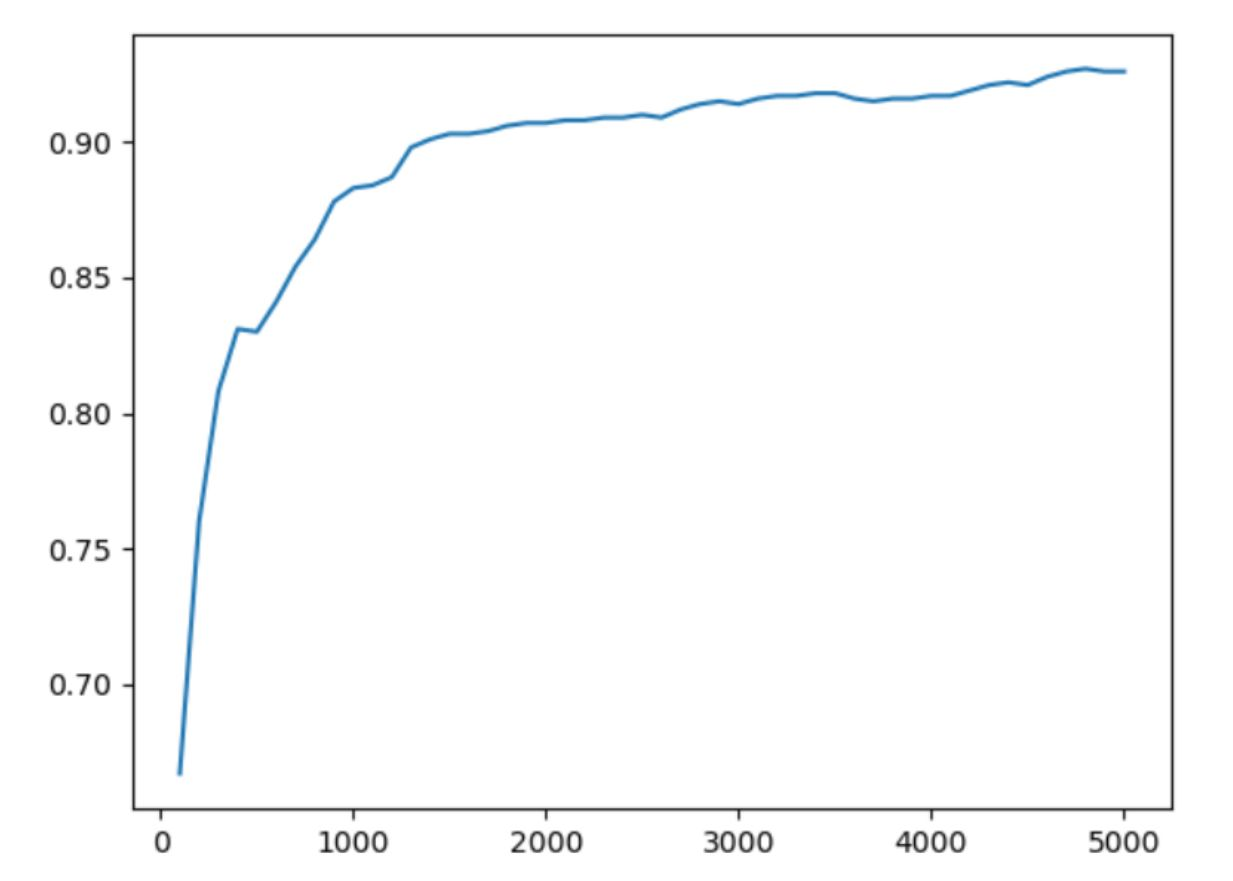
\includegraphics[scale=0.43]{plot 3.JPG}\\
 It was my first time "LaTeXing" hope it was find (:
\end{center}
\end{document}


\section*{Programming Assignment}
\subsection*{Visualizing the Hoeffding bound:}
